% Chapter 4

\chapter{Desarrollo}
\label{capitulo4}

\section{Preperaciones del Ambiente de Desarrollo}

\subsection{Sistema Base de Desarrollo}

\begin{figure}
	\begin{center}
    	%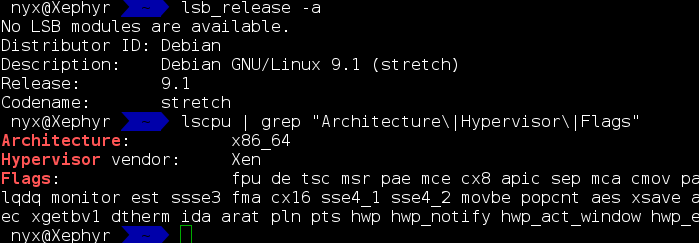
\includegraphics[width=0.5\textwidth]{Figures/sistema-base.png}
    \end{center}
  	\caption{Información del Sistema Base.}
    \label{sistema-base}
\end{figure}

El sistema base para el desarrollo de este trabajo de titulacion fue realizado con Xen instalado con Debian Stretch (9.1) instalado en un LVM con el nombre del grupo de volumenes ''Xephyr-VG''. Originalmente se tenia planificado trabajar con Debian Jessie (8.x) debido que eso fue la version estable al momento de instalacion pero despues se opto por una actualizacion a la version beta de Debian en aquello momento (Debian Stretch). En resumen los pasos realizados fueron:
\lstset{language=Bash}
\begin{enumerate}
	\item Instalacion Limpia de Debian 8 con un LVM.
    \item Actualizar Instalacion de Debian 8.
    	\begin{lstlisting}
    apt update
    apt upgrade
    apt dist-upgrade
    reboot
        \end{lstlisting}
    \item Actualizar Debian 8 a Debian 9.
        \begin{lstlisting}
    sed -i 's/jessie/stretch/g' /etc/apt/sources.list
    apt update
    apt upgrade
    reboot
        \end{lstlisting}
    \item Instalacion de Herramientas de Trabajo
        \begin{lstlisting}
    apt tmux vim zsh
        \end{lstlisting}
    \item Instalacion y Configuracion de Hipervisor Xen
		\begin{lstlisting}
    apt install tmux vim zsh
    apt install xen-hypervisor
    dpkg-divert --divert /etc/grub.d/08_linux_xen --rename /etc/grub.d/20_linux_xen
    update-grub
    cat > /etc/network/interfaces.d/xenbr << EOF

    auto xenbr0
    iface xenbr0 inet static
       address 10.10.10.1
       netmask 255.255.255.0
       bridge_ports wlan0

    #other possibly useful options in a virtualized environment
      #bridge_stp off       # disable Spanning Tree Protocol
      #bridge_waitport 0    # no delay before a port becomes available
      #bridge_fd 0          # no forwarding delay

    ## configure a (separate) bridge for the DomUs without giving Dom0 an IP on it
    #auto xenbr1
    #iface xenbr1 inet manual
    #   bridge_ports eth1

    EOF

    reboot
		\end{lstlisting}
	\item Instalacion de Herramientas de Xen
		\begin{lstlisting}
	apt install xen-tools xen-utils
		\end{lstlisting}
\end{enumerate}

Estos pasos de instalacion se basaron en la guia de instalacion de Xen publicado en el wiki del proyecto de Debian \citep{Debian-Wiki-Xen}.

\subsection{Moodle}

\section{GitEDU}

\subsection{Autenticacion por LTI}

\subsection{Editor de Codigo en Linea}

\subsection{Persistencia de Codigo}

\subsection{Sincronizacion de Notas por LTI}

\subsection{API Externa}

\section{EduNube}

\subsection{Ejeccucion de Codigo en Linea}

\subsection{Calificacion Automatizada con Pruebas Unitarias}

\subsection{API Externa}
